We measure the percentage of privacy policies updated each interval.
To determine if these changes align with shifts in the language of privacy policies, we measure the number of terms that have experienced changes in their usage at each interval.

\textbf{Privacy policy updates.}
\label{sec:policy-updates}
\begin{figure}[]
\centering
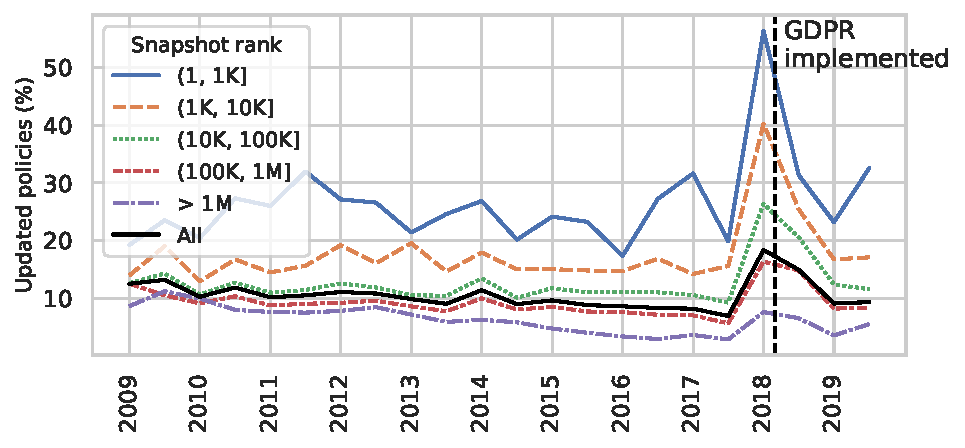
\includegraphics[width=0.99\columnwidth]{figures/policy-updates.pdf}
\caption[Caption]{Percentage of privacy policies updated per interval.\protect\footnotemark}
\label{fig:pct-policy-update}
\end{figure}
\footnotetext{We excluded snapshots for which we have a gap in the previous interval from Figure~\ref{fig:pct-policy-update}, since determining the exact time of the updates was not possible.}
Figure~\ref{fig:pct-policy-update} shows the percentage of updated policies, considering
only the~\emph{significant} updates, where the fuzzy similarity ratio~\cite{fuzzywuzzy} of consecutive policy snapshots is less than or equal to 95\%
~\cite{linden2020privacy}.
The spike in 2018 indicates the GDPR's substantial impact on privacy policies.  Although the figure shows that
popular websites update their policies more frequently,
the GDPR appears to have caused a major uptick across all rank buckets. 





\textbf{Change-point concentration.} 
To 
investigate the changes in the privacy policy language and vocabulary,
we counted the number of n-gram frequency change-points detected by the PELT algorithm~\cite{killick2012optimal}, using the \textit{ruptures} library~\cite{ruptures}. Change point detection algorithms originate from the signal processing literature, and are designed to identify when a time-series signal has experienced a failure~\cite{picard1985testing}. In our case, n-gram frequency is the signal, and the ``failures'' are events that cause a shift in the usage.


We counted the number of change-points at each interval for lemmatized 1-grams and 8-grams with a document frequency of at least $0.01$ in at least one interval.
Figure~\ref{fig:changepoints} shows that the change points for n-grams concentrate around GDPR's introduction, following a similar trend to document level updates in Figure~\ref{fig:pct-policy-update}. This indicates that not only are websites updating their policies, but that the vocabulary used in privacy policies was forced to evolve due to the GDPR.


\textbf{Validation.} To verify that the increase in privacy policy updates we observed in 2018A was related to the GDPR, we took a list of GDPR-related phrases identified by Degeling et al.~\cite{degeling2018we}, plus the phrases “GDPR” and “General Data Protection Regulation,” and selected the subset of 20 phrases with a relative document frequency of less than 1\% in 2015A. We found that documents in 2018A containing at least one of these 20 GDPR-related phrases had a mean update length of 136 new lines, compared to 15 new lines in documents without these phrases, where “update length” is the number of added lines minus the number of deleted lines. The quartile boundaries were at, respectively, 0, 20, 129 and 0, 0, 0. This indicates that policies that contain GDPR-related terms were more likely to have a longer update in comparison to the prior version of the policy, supporting the link between the introduction of the GDPR and the increase in updates in 2018A.

\begin{figure}
    \centering
    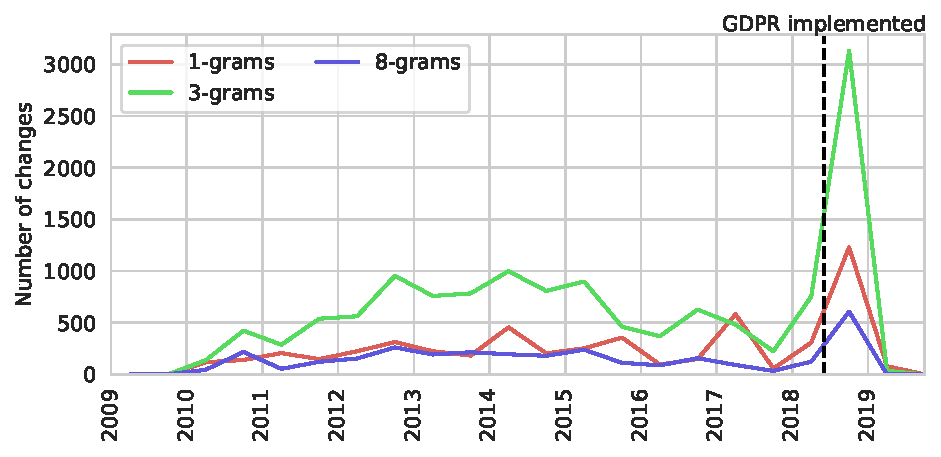
\includegraphics[width=0.45\textwidth]{figures/changepoints.pdf}
    \caption{Change point concentration. The y value is the number of frequent n-grams with change points in that interval for 1-grams and 8-grams.}
    \label{fig:changepoints}
\end{figure}
